%
\documentclass[12pt]{article}

\usepackage{fullpage}
\usepackage{setspace}
\usepackage{endnotes}
\usepackage{amsmath}
\usepackage{amsfonts}
\usepackage{amssymb}
\usepackage{rotating}
\usepackage{dcolumn}
\usepackage{longtable}
\usepackage{microtype}
\usepackage{graphicx}
\usepackage{url}
\usepackage{natbib}
\bibpunct{(}{)}{;}{a}{}{,}
\usepackage{framed}
\usepackage{lipsum}
\usepackage[font=small,labelfont=sc]{caption}
 \usepackage{float}
\restylefloat{table}
\usepackage[usenames,dvipsnames]{color}

% refs and pdf meta
\usepackage{hyperref}
\hypersetup{
 pdftitle={Reasonable Measures of Uncertainty Under Separation}, % title
 pdfauthor={Carlisle Rainey}, % author
 pdfkeywords={logistic regression}{separation}{Firth}{Cauchy}{MCMC}
 pdfnewwindow=true, % links in new window
 colorlinks=true, % false: boxed links; true: colored links
 linkcolor=BrickRed, % color of internal links
 citecolor=BrickRed, % color of links to bibliography
 filecolor=BrickRed, % color of file links
 urlcolor=BrickRed % color of external links
}

% Set up theorems, etc.
\usepackage{amsthm}
\newtheorem{lemma}{Lemma}
\newtheorem{proposition}{Proposition}
\newtheorem{theorem}{Theorem}
\newtheorem{claim}{Claim}
\newtheorem{assumption}{Assumption}

% Allow restating theorems (for the Appendix)
\usepackage{thmtools}
\usepackage{thm-restate}
\usepackage{cleveref}


% Set up fonts the way I like
\usepackage{tgpagella}
\usepackage[T1]{fontenc}
%\usepackage[T1]{fontenc}
\usepackage[bitstream-charter]{mathdesign}


%Redefine the first level
\renewcommand{\theenumi}{\arabic{enumi}.}
\renewcommand{\labelenumi}{\theenumi}
%Redefine the second level
\renewcommand{\theenumii}{\alph{enumii}.}
\renewcommand{\labelenumii}{\theenumii}
%Redefine the third level
\renewcommand{\theenumiii}{\roman{enumiii}.}
\renewcommand{\labelenumiii}{\theenumiii}
%Redefine the fourth level
\renewcommand{\theenumiv}{\Alph{enumiv}.}
\renewcommand{\labelenumiv}{\theenumiv}


\parskip=0pt
\parindent=20pt
\usepackage{lscape}
\singlespace

% Create footnote command so that my name
% has an asterisk rather than a one.
\long\def\symbolfootnote[#1]#2{\begingroup%
\def\thefootnote{\fnsymbol{footnote}}\footnote[#1]{#2}\endgroup}

\begin{document}


\begin{center}
{\LARGE Reasonable Measures of Uncertainty Under Separation\symbolfootnote[1]{I thank [many people]. Thanks to Mark Bell and Nicholas Miller for making their data available to me. The analyses presented here were conducted with \texttt{R} 3.1.0 and JAGS 3.3.0. All data and computer code necessary for replication are available at \href{https://github.com/carlislerainey/priors.for-separation}{github.com/carlislerainey/priors-for-separation}.}}

\vspace{10mm}

Carlisle Rainey\symbolfootnote[2]{Carlisle Rainey is Assistant Professor of Political Science, University at Buffalo, SUNY, 520 Park Hall, Buffalo, NY 14260 (\href{mailto:rcrainey@buffalo.edu}{rcrainey@buffalo.edu}).}

\end{center}

% remove page number from first page
\thispagestyle{empty}

% abstract
\vspace{10mm}
{\centerline{\textsc{Abstract}}}
\begin{quote}\noindent When facing data sets with small numbers of observations or ``rare events,'' political scientists often encounter important explanatory variables that perfectly predict binary events or non-events. In this situation, maximum likelihood provides implausible estimates and the researcher must incorporate some form of prior information in the estimation. The most sophisticated research uses Jeffreys' invariant prior to stabilize the estimates. While Jeffreys' prior has the advantage of being automatic, I show that, in many cases, it offers too much prior information, providing confidence intervals that are much too narrow. I show that the choice of a more reasonable prior can lead to different substantive conclusions about the likely magnitude of an effect and I offer practice advice for choosing a prior distribution that represents actual prior information.\end{quote}


\newpage
\doublespace

\section*{The Logistic Regression Model}

Political scientists commonly use logistic regression to model the probability of an event of interest. In the typical situation, the researcher uses an $n \times k + 1$ design matrix $X$ consisting of an intercept and $k$ covariates to model a vector $n$ of binary outcomes $y$, where $y_i \in \{0, 1\}$ using the model $\text{Pr}(y_i) = \text{Pr}(y_i = 1 | X) = \dfrac{1}{1 + e^{-X_i\beta}}$, where $\beta$ is a parameter vector of length $k + 1$. 

Using this model, it is straightforward to calculate the likelihood function 

\begin{equation}\nonumber
\text{Pr}(y | \beta) = L(\beta | y) = \displaystyle \prod_{i = 1}^n \left[\left( \dfrac{1}{1 + e^{-X_i\beta}}\right)^{y_i} + \left( \dfrac{1}{1 + e^{-X_i\beta}}\right)^{1 - y_i}\right]\text{.}
\end{equation}

\noindent As usual, one can take the natural logarithm of both sides to calculate the log-likelihood function 

\begin{equation}\nonumber
\log L(\beta | y) = \displaystyle \sum_{i = 1}^n \left[y_i \log \left( \dfrac{1}{1 + e^{-X_i\beta}}\right) + (1 - y_i) \log \left( \dfrac{1}{1 + e^{-X_i\beta}}\right)\right]
\end{equation}

\noindent and take the derivatives of the log-likelihood function to obtain the score function

\begin{equation}\nonumber
\dfrac{\partial \log L(\beta | y)}{\partial \beta} = \displaystyle \sum_{i = 1}^n\left(y_i - \dfrac{1}{1 + e^{-X_i\beta}}\right)X_i\text{.}
\end{equation}

Researchers routinely obtain estimates $\hat{\beta}$ of the model parameters $\beta$ by setting the score function equal to zero and solving for $\beta$ (i.e., maximizing the likelihood of the observed data) and estimate the standard errors are by calculating the square root of the diagonal of the inverse of Fisher's information matrix evaluated at $\hat{\beta}$ (i.e., calculate the curvature around the maximum of the likelihood function to obtain an estimate of the uncertainty of the estimate). While this approach works quite well in most applications, it fails in a situation known as separation \citep{Zorn2005}.

\section*{The Importance of the Prior}

Choosing a reasonable prior distribution is crucial for dealing with separation in a substantively meaningful manner. In many cases, the data (though the likelihood) swamp the contribution of the prior. However, in the case of separation such that $s_i$ perfectly predicts events, the likelihood determines the shape of the left-hand side of the posterior distribution and the prior (symmetric about zero) determines the shape of the right hand side of the posterior.

The likelihood has an ``S''-shape that approaches a limit of one as the parameter $\beta_s$ for the separating variable $s$ approaches infinity. Thus, for large values of $\beta_s$, the likelihood is essentially flat, which allows the prior distribution to drive the inferences. Thus the prior distribution is not an arbitrary choice made for computational convenience--but a choice that affects the inferences.

\subsection*{The Impact of the Prior in Theory}

Suppose that an explanatory variable $s_i$ perfectly predicts a binary outcome variable $y_i = 1$, such that whenever $s_i = 1$, $y_i = 1$, but when $s_i = 0$, $y_i$ might equal zero or one. \cite{AlbertAnderson1984} refer to this situation as quasicomplete separation. Suppose further an additional set of covariates $X_i$ and the analyst wishes to obtain plausible estimates of coefficients the model $Pr(y_i =1) = \text{logit}^{-1}(\alpha + \beta s_i + X_i \gamma)$. It is easy to find plausible estimates of $\gamma$ using the techniques discussed above (even maximum likelihood usually provides reasonable estimates of these parameters), but finding plausible estimates of $\alpha$ and $\beta$ proves more difficult because maximum likelihood suggests estimates of $-\infty$ and $+\infty$, respectively. In order to obtain a plausible estimate of $\beta$ (which will, in turn, provide a plausible estimate of $\alpha$), the researcher must introduce prior information into the model. My purpose here is to characterize how this prior information impacts the posterior distribution.

In the general situation, the analyst is interested in computing and characterizing the posterior distribution of the coefficient for $s_i$ given the data. Using Bayes' Rule, this posterior depends on the likelihood and the prior, so that $p(\beta | y) = p(y|\beta)p(\beta)$. In particular, the analyst might have in mind a family of priors centered at and monotonically decreasing away from zero with varying scale $\sigma$, so that $p(\beta) = p(\beta|\sigma)$. Suppose that for a particular $\beta^* \geq 0$ the prior distribution is decreasing in $\beta$ at a decreasing rate. Intuitively, this assumption of a $\beta^*$ allows the result to generalize to many common distributions.\footnote{In particular, if the prior distribution is in the form of a double-exponential, which lacks ``shoulders,'' then $\beta^* = 0$. However, the most common prior distributions used in applied work, such as the normal, $t$, and Jeffreys', have ``shoulders'' such that $\beta^* > 0$. In this case, the exact curvature of the distribution in the region $[0, \beta^*]$ affects the relative impact of the prior.} 
Finally, suppose that the informativeness of the prior distribution depends on scale parameter $\sigma$ that is chosen by the researcher and ``flattens'' the prior $p(\beta) = p(\beta | \sigma)$, such that as $\sigma$ increases, the rate a which the prior descends to zero decreases.

\begin{restatable}{theorem}{impact}\label{thm:impact}
The impact of the researchers choice of $\sigma$ on the posterior distribution $p(\beta | y)$ is increasing in $\beta$ for $\beta> \beta^*$. 
\end{restatable}

In many cases, researchers summarize the posterior distribution by providing the 5th and 95th percentiles and a measure of centrality, such as the median.

\begin{quote}
\textsc{Practical Implication of Theorem \ref{thm:impact}:} Under quasicomplete separation where $x_i$ perfectly predicts $y_i = 1$, the prior has a small impact on the lower bound of the 90\% credible interval, a moderate impact on the measures of the location of the posterior (i.e., mean, median, and mode), and a large impact on the upper-bound of the credible interval.
\end{quote}

\subsection*{The Impact of the Prior in Practice}

To illustrate the impact of the prior on inferences when facing separation, I replicate a results from \cite{BarrilleauxRainey2014}, who are interesting in the effect of partisanship on governors' decisions to oppose the Medicaid expansion in their states under the Patient Protection and Affordable Care Act (ACA).\footnote{\cite{BarrilleauxRainey2014} use a logistic regression modeling the probability that a governor opposes the expansion using the following explanatory variables: the partisanship of the governor, the percent of the state's residents who are favorable toward the ACA, whether Republicans control the state legislature, the percent of the state that is uninsured, a measure of the fiscal health of the state, the Medicaid multiplier for the state, the percent of the state that is nonwhite, and the percent of the state that resides in a metropolitan area. See their paper for more details.} As the authors note, no Democrats opposed the expansion leading to a problem of separation. I use MCMC to simulate from the posterior using several different prior distributions, including Jeffreys' prior \citep{Zorn2005} and the Cauchy prior with scales of 1, 2.5, and 5 \citep{Gelmanetal2008}. While the choice of prior does not affect the conclusion about the \emph{direction} of the effect, it has a large impact on the conclusion about the \emph{magnitude} of the effect. This can be especially important when researchers are making claims about the substantive importance of their estimated effects (see \citealt{Rainey2014}, \citealt{Gross2014}, and \citealt{McCaskeyRainey2014}).

Figure \ref{fig:matters-post} shows the posterior distribution for the coefficient for the indicator of Republican governors. Notice that the different priors lead to different posterior distributions. Notice, in particular, that the choice of the prior has a large impact on the right-hand side of the posterior. More informative priors (e.g., Jeffrey's prior) lead to a more peaked posterior distribution that rules out very large effects. Less informative priors (e.g., Cauchy(2.5)) lead to the conclusion that even large effects are plausible. These differences affect the conclusions that the researchers draw about the likely magnitude of the effect.

\begin{figure}[H]
\begin{center}
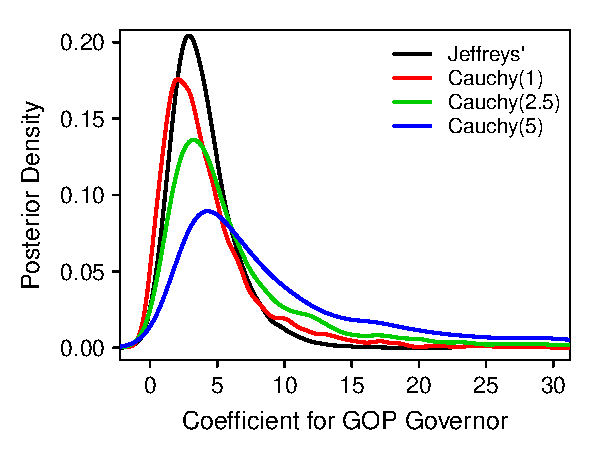
\includegraphics[scale = .8]{figs/matters-post.pdf}
\caption{This figure provides the posterior distribution for the coefficient of the indicator for GOP governors in the model offered by \cite{BarrilleauxRainey2014}. Notice that the location and the spread of the posterior depend on the prior chosen, especially the right-hand side of the distribution.}\label{fig:matters-post}
\end{center}
\end{figure}

Figure \ref{fig:matters-ci} shows how the choice of prior impacts the 90\% credible interval. Notice that different prior distributions lead to different conclusions about the plausible values of the effect. In particular, different priors lead to different conclusions about the upper-bound on the plausible effect sizes. For example, Jeffreys' prior, the default proposed by \cite{Zorn2005} and \cite{HeinzeSchemper2002}, suggests the effect lies in the range $\beta_{\text{GOP Gov.}} \in [0.9, 8.4]$, with a posterior mean of 3.9. On the other hand, the less informative Cauchy(2.5) prior, the default proposed by \cite{Gelmanetal2008}, suggests the effect lies in the range $\beta_{\text{GOP Gov.}} \in [1.0, 22.5]$, with a posterior mean of 7.3. A simple change from one proposed default to another more than doubles the upper bound on the 90\% credible interval and almost doubles the posterior mean. Further, the Cauchy(5) prior, a plausible prior if one believes the effect might be large, produces the upper-bound on the 90\% credible interval from is more than four times larger than the upper-bound produced by Jeffrey's prior. The posterior mean from the Cauchy(5) prior is larger falls above the upper-bound from the 90\% credible interval from Jeffrey's prior.

\begin{figure}[H]
\begin{center}
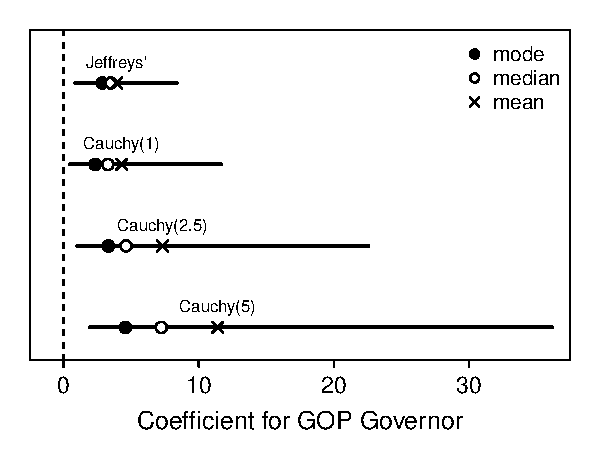
\includegraphics[scale = .8]{figs/matters-ci.pdf}
\caption{This figure provides the (equal-tailed) 90\% credible intervals for the coefficient of the indicator for GOP governors in the model offered by \cite{BarrilleauxRainey2014}. Notice that the location and the spread of the posterior depend on the prior chosen, especially the right-hand side of the distribution. Note that Jeffrey's prior, suggested by \cite{Zorn2005}, is the most informative of these priors, suggesting that a coefficient smaller than about 10 is quite unlikely. On the other hand, credible interval using the Cauchy(2.5) prior, as suggested by \cite{Gelmanetal2008}, is about \emph{twice} as wide as the credible interval from Jeffreys' prior. Finally, notice that the Cauchy(5) prior--a plausible prior if the researcher believes the effect might be large--produces a posterior mean larger than the upper bound of the 90\% credible interval using Jeffrey's prior.}\label{fig:matters-ci}
\end{center}
\end{figure}

This leads us to conclude that the choice of prior matters--it affects the inferences that we draw from the data. It is not sufficient to rely on the prior distribution designed as a default for other purposes. Instead, we must rely on prior distributions that represent actual prior information about the likely magnitude of the coefficients.

\clearpage
\bibliographystyle{apsr_fs}
\bibliography{/Users/carlislerainey/Dropbox/papers/bibliography/bibliography.bib}

\clearpage
\begin{appendix}
\begin{center}
\LARGE{\textbf{Online Appendix}}\vspace{4mm}
\end{center}

\section*{Proof of Theorem \ref{thm:impact}}

\begin{assumption}[Separation]
Suppose quasicomplete separation such that $s_i$ perfectly predicts $y_i = 1$. 
\end{assumption}

\begin{assumption}[Prior Shape]
Suppose that the researcher computes the posterior distribution $p(\beta | y) = p(y | \beta)p(\beta)$ such that for a particular $\beta^* \geq 0$ the prior distribution is decreasing at a decreasing rate.
\end{assumption}

Intuitively, this assumption of a $\beta^*$ allows the result to generalize to a range of common distributions. In particular, if the prior distribution is in the form of a double-exponential, which lacks ``shoulders,'' then $\beta^* = 0$. However, the most common prior distributions used in applied work, such as the normal, $t$, and Jeffreys', have ``shoulders'' such that $\beta^* > 0$. In this case, the exact curvature of the distribution in the region $[0, \beta^*]$ affects the relative impact of the prior.

\begin{assumption}[Scale Parameter]
Suppose finally the that informativeness of the prior distribution depends on scale parameter $\sigma$ ``flattens'' the prior $p(\beta) = p(\beta | \sigma)$, such that as $\sigma$ increases, the rate a which the prior descends to zero decreases.
\end{assumption}

$\sigma$ is chosen by the researcher based on prior information about the likely values of the coefficients.

Before proving Theorem \ref{thm:impact}, it is helpful to show several initial results.

\begin{lemma}\label{thm:L1}
$\dfrac{\partial p(y | \beta)}{\partial \beta} > 0$ for all $\beta$. 
\end{lemma}

\begin{proof}[Proof of Lemma \ref{thm:L1}]
The quantity $p(y | \beta)$ is the probability of observing $y$ (i.e., an outcome variable separated by $s$). Increasing values of $\beta$ make this separation increasingly likely. Thus, $p(y | \beta)$ is increasing in $\beta$ so that $\dfrac{\partial p(y | \beta)}{\partial \beta} > 0$. 
\end{proof}

\begin{lemma}\label{thm:L2}
$p(\beta | \sigma) > 0$ for all $\beta$.
\end{lemma}

\begin{proof}[Proof of Lemma \ref{thm:L2}]
The quantity $p(\beta | \sigma)$ is a probability distribution defined to have support over the real line and thus $p(\beta | \sigma) > 0$ for all $\beta$. 
\end{proof}

\begin{lemma}\label{thm:L3}
$p(y | \beta) > 0$ for all $\beta$.
\end{lemma}

\begin{proof}[Proof of Lemma \ref{thm:L3}]
The quantity $p(y | \beta)$ is a probability and thus bounded between zero and one. As long as data lie within the support of the probability model, this quantity lies strictly above zero. Since the theorem defines the data as such, $p(y | \beta) > 0$.
\end{proof}

\begin{lemma}\label{thm:L4}
$\dfrac{\partial^2 p(\beta | \sigma)}{\partial \beta \partial \sigma}$ for $\beta > \beta^*$.
\end{lemma}

\begin{proof}[Proof of Lemma \ref{thm:L4}]
By assumption, the prior density is decreasing at a decreasing rate in $\beta$ for all $\beta > \beta^*$. Also by assumption, the scale parameter $\sigma$ controls the rate at which $\beta$ decreases such that increasing $\sigma$ leads to a slower rate of decrease. These two assumptions together imply that $\dfrac{\partial^2 p(\beta | \sigma)}{\partial \beta \partial \sigma}$ for $\beta > \beta^*$.
\end{proof}

Now recall Theorem \ref{thm:impact}:

\impact*

\begin{proof}[Proof of Theorem \ref{thm:impact}]
To show that the effect of $\sigma$ is increasing in $\beta$, I simply need to show that $\dfrac{\partial^2 p(\beta | y)}{\partial \beta \partial \sigma} > 0$ for $\beta > \beta^*$. 

Recall that the posterior $p(\beta | y)$ is proportional to the likelihood $p(y | \beta)$ times the prior $\beta(\beta | \sigma)$, so that $p(\beta | y) \propto p(y|\beta)p(\beta | \sigma)$. First, we can use the product rule to obtain the derivative of $p(\beta | y)$ so that 

\begin{equation}\nonumber
\dfrac{\partial p(\beta | y)}{\partial \beta} \propto \dfrac{\partial p(y | \beta)}{\partial \beta} p(\beta | \sigma) + p(y | \beta)\dfrac{\partial p(\beta | \sigma)}{\partial \beta \partial}\text{}.
\end{equation}

\noindent Only the final term involves $\sigma$, so we can easily obtain the desired derivative

\begin{equation}\label{eqn:cross-partial}
\dfrac{\partial^2 p(\beta | y)}{\partial \beta \partial \sigma} \propto \overbrace{\dfrac{\partial p(y | \beta)}{\partial \beta}}^{\text{Lemma 1}:~+} \overbrace{p(\beta | \sigma)}^{\text{Lemma 2}:~+} + \overbrace{p(y | \beta)}^{\text{Lemma 3}:~+} \overbrace{\dfrac{\partial^2 p(\beta | \sigma)}{\partial \beta \partial \sigma}}^{\text{Lemma 4}:~+}\text{.}
\end{equation}

\noindent Each term on the right-hand side of Equation \ref{eqn:cross-partial} is positive  for $\beta > \beta^*$ (Lemmas 1-4), so that $\dfrac{\partial^2 p(\beta | y)}{\partial \beta \partial \sigma} > 0$ for $\beta > \beta^*$.

\end{proof}

\end{appendix}
\end{document}



